\paragraph{QuizziPedia::Back-End::App::Models::ErrorModel}
\label{QuizziPedia::Back-End::App::Models::ErrorModel}
\begin{figure}[ht]
	\centering
	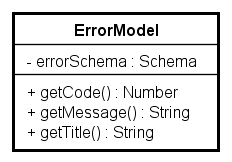
\includegraphics[scale=0.8]{UML/Classi/Back-End/QuizziPedia_Back-End_App_Models_errorModel.png}
	\caption{QuizziPedia::Back-End::App::Models::ErrorModel}
\end{figure}
\FloatBarrier
\begin{itemize}
	\item \textbf{Descrizione}: classe che rappresenta le informazioni di un errore che si è verificato eseguendo una determinata operazione;
	\item \textbf{Utilizzo}: viene utilizzata per racchiudere tutte le informazioni riguardanti l'errore;
	\item \textbf{Relazioni con altre classi}:
		\begin{itemize}
			\item \textbf{IN \texttt{ErrorHandler}} \\
			Classe \textit{middleware\ped{G}} per la gestione degli errori. Ritorna al \textit{client\ped{G}} un oggetto di tipo \texttt{Response} con stato \textit{HTTP\ped{G}} 500 e descrizione dell'errore in formato \textit{JSON\ped{G}}. È un componente \textit{ConcreteHandler\ped{G}} del \textit{design pattern\ped{G}} \textit{Chain of responsability\ped{G}}.
		\end{itemize}
	\item \textbf{Attributi}:
		\begin{itemize}
			\item \texttt{- errorSchema: Schema} \\
			Questo campo dati rappresenta lo schema \textit{Mongoose\ped{G}} per gli errori e prevede i seguenti attributi:
				\begin{itemize}
					\item \texttt{errorCode: Number}\\ Rappresenta il codice dell'errore;
					\item \texttt{errorMessage: String}\\ Rappresenta la descrizione dell'errore; 
					\item \texttt{errorTitle	: String}\\ Rappresenta il titolo del messaggio d'errore.
				\end{itemize}
		\end{itemize}
	\item \textbf{Metodi}:
		\begin{itemize}
			\item \texttt{+ getCode() : Number} \\
			Metodo che consente di ottenere il codice dell'errore;
			\item \texttt{+ getMessage() : String} \\
			Metodo che consente di ottenere la descrizione dell'errore;
			\item \texttt{+ getTitle() : String} \\
			Metodo che consente di ottenere il titolo del messaggio d'errore. 
		\end{itemize}
\end{itemize}